\chapter{Análisis estadístico}

%Teniendo los datos guardados y limpios, proseguimos con la siguiente etapa del proyecto, se realizó un análisis estadístico de los datos. Para ello se observaron los grupos de datos en los que se dividió la información, se eligió el método Holt-Winters aditivo el cual funciona para series de tiempo con componentes de tendencia aproximadamente lineal y de estacionalidad.

%Teniendo los datos guardados y limpios, se realizó un análisis estadístico de los datos, las herramientas elegidas para dicho análisis fueron las series de tiempo y el método Holt-Winters aditivo el cual funciona para series de tiempo con componentes de tendencia aproximadamente lineal y de estacionalidad.

Debido a la naturaleza de los datos, las herramientas elegidas para realizar un análisis estadístico de los datos fueron las series de tiempo. A continuación se describe su definición y aplicación para explicar el motivo de la elección de dichas herramientas estadísticas.

Definimos a una serie de tiempo como una secuencia de observaciones $X_{t}$ ordenadas cronológicamente. Los datos al tiempo presente dependen de las observaciones anteriores, es decir existe una depencia de $X_{t}$ con $\{X_{t-1}, X_{t-2}, X_{t-3}, \ldots, X_{2}, X_{1}, X_{0}, \ldots\}$.

Denotamos a una serie de tiempo como:
  \begin{equation}
X_{t} = m_{t} + s_{t} + y_{t},
\end{equation}

donde las componentes de la serie de tiempo $(m_{t}, s_{t}, y_{t})$ tienen las siguientes propiedades:

\begin{itemize}
\item[-] Tendencia $(m_{t})$: Se le llama tendencia al cambio, a largo plazo, del promedio de los datos. El cambio puede ser creciente o decreciente.

\item[-] Estacionalidad $(s_{t})$: Se llama variación estacional a las fluctuaciones periódicas que tiene una serie de tiempo. La longitud de cada periodo es constante y por lo general menor o igual a un año, por ejemplo semanal, mensual o semestral.

\item[-] Aleatoriedad $(y_{t})$: También llamada componente irregular, son series de residuales que pueden o no ser aleatorios.
\end{itemize}

Chatfield y Xing, en su libro \textit{The Analysis of Time Series An Introduction with R} [\ref{ChatfieldXing}], nos indican que existen 2 tipos de variación estacional:
  
  \begin{itemize}
\item[-] Aditiva: Se dice que la estacionalidad es aditiva cuando la longitud de cada periodo es constante año con año.

\item[-] Multiplicativa: Se dice que la estacionalidad es multiplicativa cuando la longitud de cada periodo es directamente proporcional a la media de los datos de la serie de tiempo.
\end{itemize}

Con estos tipos de variaciones se forman 3 modelos de estacionalidad:

%Se dice que una serie de tiempo es estacionaria si a lo largo del tiempo su media y su varianza con constantes y es no estacionaria si su tendencia y variabilidad cambian en el tiempo. %%No nos sirve la serie de tiempo estacionaria porque la media de nuestros datos no se mantiene constante.

  \begin{enumerate}
\item Aditivo: En este modelo se tiene variación estacional aditiva. Se utiliza cuando la varianza o la desviación estándar de la serie de tiempo se mantienen constantes a lo largo del tiempo. El modelo aditivo se denota como:
\begin{equation}
X_{t} = m_{t} + s_{t} + y_{t}.
\end{equation}

\item Multiplicativo: En este modelo se tiene variación estacional multiplicativa. Se utiliza cuando la varianza o la desviación estándar de los datos cambian a través del tiempo. Su variabilidad puede ser mayor o menor conforme pasa el tiempo. El modelo multiplicativo se denota como:
\begin{equation}
X_{t} = m_{t}s_{t}y_{t}.
\end{equation}

\item Mixto: Este modelo se utiliza cuando se tiene variación estacional multiplicativa pero la variabilidad de la componente irregular se mantiene constante a lo largo del tiempo. El modelo mixto se denota como:
\begin{equation}
X_{t} = m_{t}s_{t} + y_{t}.
\end{equation}
\end{enumerate}

Los objetivos principales al hacer el análisis de una serie de tiempo son:
  
  \begin{itemize}
\item[-] Describir: Leer datos en una tabla es mucho más tardado y en algunas ocasiones más complicado que observar una gráfica de los datos que se tienen. Las gráficas ayudan a ver de una manera más inmediata el comportamiento que tienen los datos y es posible observar si la serie de tiempo tiene alguna tendencia o estacionalidad. También se puede ver la posible falta de información o valores atípicos.

\item[-] Predecir: Teniendo una serie de tiempo se desea conocer qué va a pasar en el futuro. Es conveniente tener varios periodos de información para que la predicción sea lo más acertada posible.
\end{itemize}

Las áreas en las que se pueden aplicar las series de tiempo son por ejemplo en economía, demografía, finanzas, medio ambiente, ingeniería o medicina. En estas áreas, algunos ejemplos de su aplicación son: precios de acciones diarios, niveles de producción en la agricultura mensuales, medición del sonido por segundos, barriles de petróleo producidos al año, electrocardiogramas, medición de terremotos, tasa de mortalidad, tasa de natalidad, entre otros.


\section{Análisis estadístico básico}

En esta sección haremos un análisis básico de los datos correspondientes a las carreras del Departamento de Matemáticas. Para dicho análisis utilizamos series de tiempo. Con la función \verb@ts()@ de \textit{R}, convertimos los datos del número total de alumnos, en una serie de tiempo. En la serie hay un dato para cada semestre del 2008-1 al 2020-1. Aplicamos la función \verb@decompose()@ a la serie de tiempo creada. Esta función utiliza el método de promedios móviles para descomponer la serie. Con ésto, obtuvimos un objeto de la clase \textit{decomposed.ts} de \textit{R}. A este objeto lo llamamos \textit{num\_total\_alum.Comp}. Los elementos que tiene \textit{num\_total\_alum.Comp} son los siguientes:

\begin{itemize}
\item[-] \textit{x:} Los valores observados de la serie de tiempo $(X_{t})$.

\item[-] \textit{seasonal:} Valores estimados de la componente estacional de la serie de tiempo $(\hat{s}_{t})$.

\item[-] \textit{figure:} Vector con los promedios del efecto estacional. La longitud del vector es igual a la frecuencia de los datos en la serie de tiempo. En este caso la longitud es $2$ porque los datos son semestrales.

\item[-] \textit{trend:} Valores estimados de la componente de tendencia $(\hat{m}_{t})$.

\item[-] \textit{random:} Valores estimados de la componente irregular $(\hat{y}_{t})$.

\item[-] \textit{type:} Tipo de variación estacional \textit{(``additive'')}.
\end{itemize}

%se pueden ver en la \figurename{~\ref{componentes_ts_totalAlum}}.
%\begin{figure}[H]
%\centering
%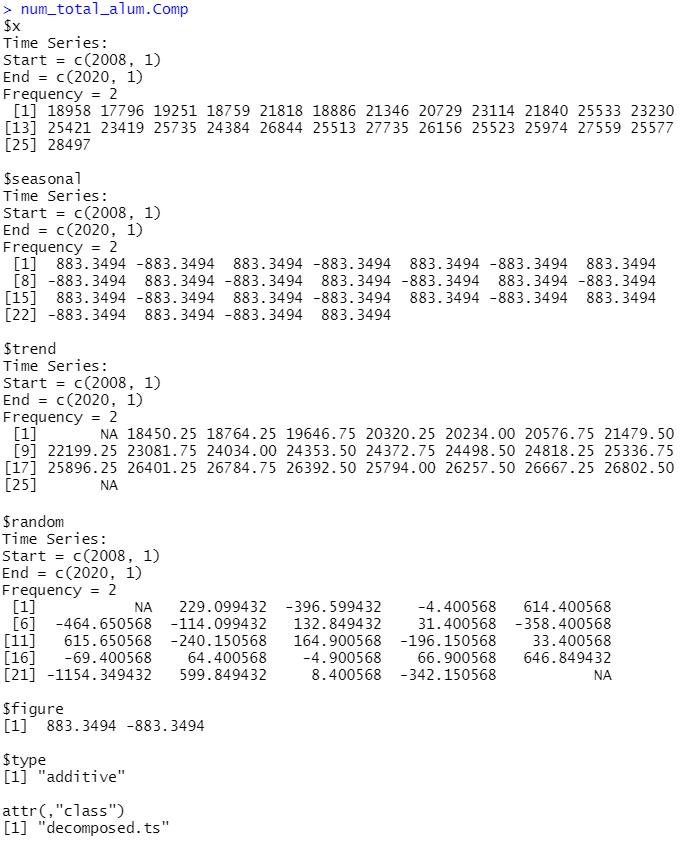
\includegraphics[width=\textwidth]{componentes_ts_total_alumnos} %scale = 0.8
%\caption[\textit{Componentes de la serie de tiempo con el número total de alumnos}]{\textit{Componentes de la serie de tiempo con el número total de alumnos...}}\label{componentes_ts_totalAlum}
%\end{figure}

Graficamos \textit{num\_total\_alum.Comp} para poder ver las componentes de la serie de tiempo (ver \figurename{~\ref{img_en_ing_2}}). Se observan 4 diferentes gráficas , en la primera, de arriba hacia abajo, se observan los datos reales del número total de alumnos para cada semestre $(X_{t})$. En la segunda se muestra $\hat{m}_{t}$, la cual notamos que es creciente. En la tercera vemos $\hat{s}_{t}$ que nos indica que los datos tienen una estacionalidad semestral. En la cuarta se ve $\hat{y}_{t}$, la cual ya no tiene estacionalidad ni tendencia.

\begin{figure}[H]
\centering
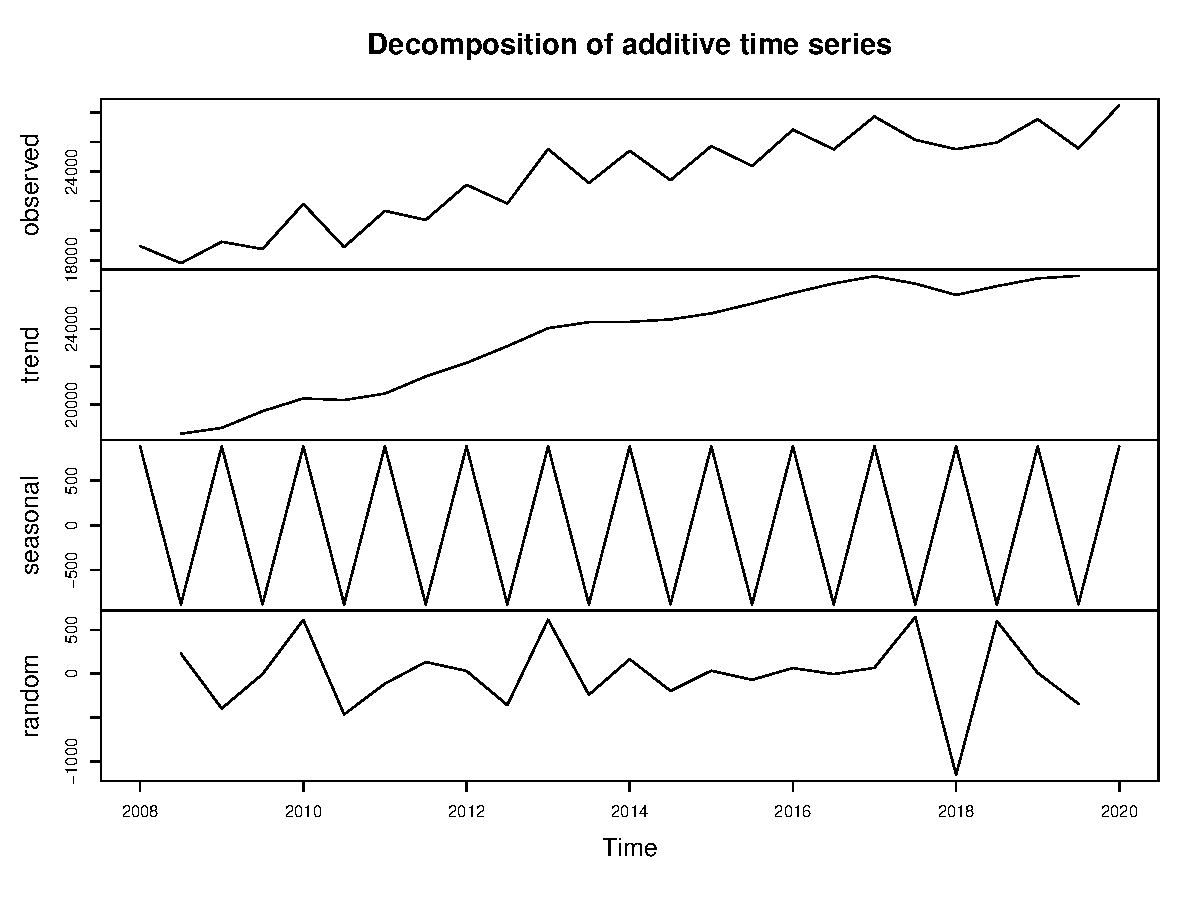
\includegraphics[width=\textwidth]{descomposicion_ts_total_alumnos.pdf} %scale = 0.8
\caption[\textit{Descomposición por el método aditivo de Holt-Winters}]{\textit{Descomposición por el método aditivo de Holt-Winters: Los datos considerados en esta descomposición es el número total de alumnos por semestre.}}\label{img_en_ing_2}
\end{figure}

Las técnicas de suavizamiento de series de tiempo son útiles para mostrar patrones subyacentes en los datos de las series de tiempo. El método que vamos a utilizar para mostrar dichos patrones de los datos es el método Holt-Winters aditivo. Este método se utiliza para describir y predecir valores con series de tiempo que tienen componentes de tendencia lineal y de estacionalidad.

Para probar éstos supuestos, existen diversas pruebas estadísticas. En las siguientes subsecciones veremos algunas de ellas. En cada una de las subsecciones presentaremos algunas gráficas de series de tiempo y otras de sus valores acumulados. Con ellas observaremos el comportamiento de los datos. Con ésto comprobaremos que los datos cumplen con los supuestos del método.


\subsection{Prueba de tendencia}

Al inicio de este capítulo vimos que se le llama tendencia al cambio, a largo plazo, del promedio de los datos. En la \figurename{~\ref{prom_alum_x_sem_ts}} se muestran las gráficas del promedio del número de alumnos que toman clases por semestre de todas las materias. En la subfigura izquierda los datos están graficados como serie de tiempo. En la subfigura derecha la línea roja representa el ajuste de la tendencia, con un modelo de regresión lineal.

Observamos que los valores tienen una tendencia creciente, ésto nos indica que cada semestre, en promedio, el número de alumnos incrementa en la Facultad.

\begin{figure}[H]
\centering
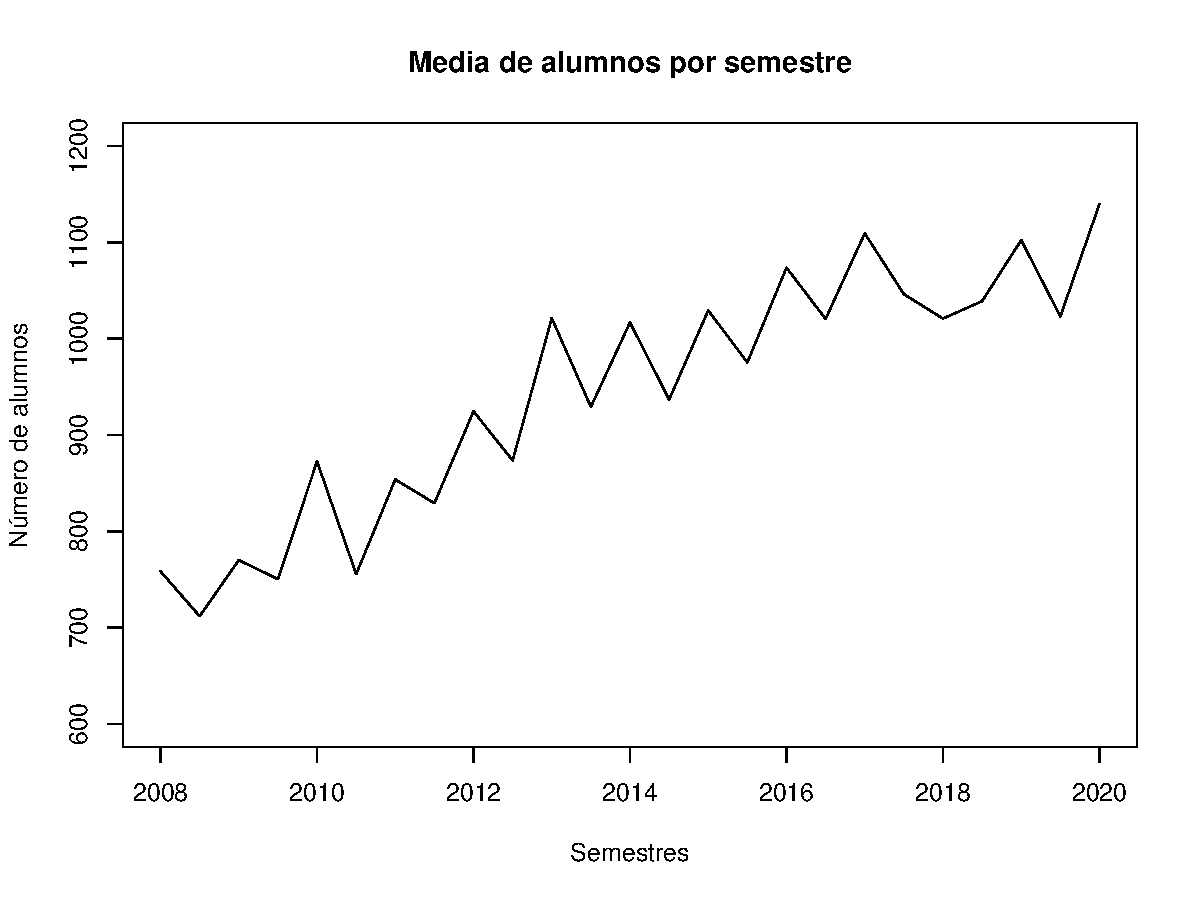
\includegraphics[width=\textwidth]{prom_alum_total_x_sem_ts.pdf} %scale = 0.7
\caption[\textit{Media de alumnos por semestre}]{\textit{Media de alumnos por semestre: Se observa una tendencia creciente en la media de alumnos por semestre. La información corresponde a los semestres del 2008-1 al 2020-1.}}\label{prom_alum_x_sem_ts}
\end{figure}

Para probar que los datos no son aleatorios utilizamos la función \verb@cox.stuart.test(X)@, de \textit{R}. Dicha función tiene como hipótesis nula $H_{0}:$ Los datos provienen de una muestra aleatoria. En la \figurename{~\ref{coxStuartTest_randomness}} se muestran los resultados de la prueba Cox-Stuart.

\begin{figure}[H]
\centering
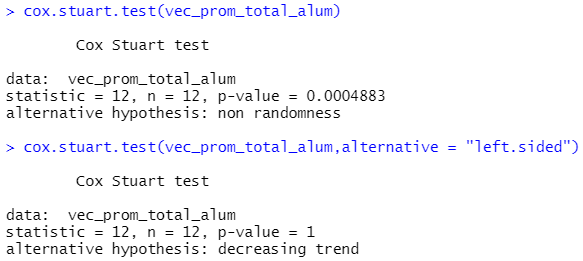
\includegraphics[scale = 1]{cox_stuart_test_randomness} %width=\textwidth
\caption[\textit{Prueba Cox-Stuart para aleatoriedad}]{\textit{Prueba Cox-Stuart para aleatoriedad: En esta figura se muestran los resultados de la prueba Cox-Stuart. Esta prueba se utiliza para probar la aleatoriedad de los datos.}}\label{coxStuartTest_randomness}
\end{figure}

Por [\ref{Casella}] sabemos que se rechaza $H_{0}$ si \textit{p-value} $ \leqslant \alpha$, siendo $\alpha$ el nivel de significancia. Sea $\alpha = 0.01$. Como vemos en la \figurename{~\ref{coxStuartTest_randomness}},  \textit{p-value} $ = 0.0004 \leqslant 0.01 = \alpha$, por lo tanto se rechaza la hipótesis nula. Con ésto podemos concluir que los datos no provienen de una muestra aleatoria. Ésto nos indica que los datos pueden tener una tendencia creciente o decreciente.

Para probar que los datos tienen una tendencia creciente utilizamos la misma prueba pero con otra alternativa. El comando en \textit{R} es: \verb@cox.stuart.test(X,alternative="left.sided")@. En la \figurename{~\ref{coxStuartTest_trend}} se muestran los resultados de la prueba. Dicha prueba tiene como hipótesis nula $H_{0}:$ Los datos tienen una tendencia creciente.

\begin{figure}[H]
\centering
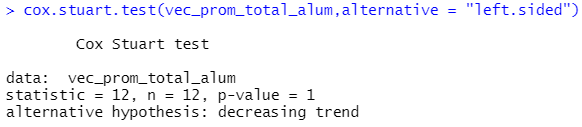
\includegraphics[scale = 1]{cox_stuart_test_increasing_trend} %width=\textwidth
\caption[\textit{Prueba Cox-Stuart para tendencia}]{\textit{Prueba Cox-Stuart para tendencia: En esta figura se muestran los resultados de la prueba Cox-Stuart para tendencia. Con la alternativa elegida, esta prueba se utiliza para probar si los datos tienen una tendencia creciente.}}\label{coxStuartTest_trend}
\end{figure}

Podemos ver en la \figurename{~\ref{coxStuartTest_trend}} que \textit{p-value} $ = 1 > 0.01 = \alpha$ por lo tanto no se rechaza $H_{0}$. Con ello concluimos que los datos tienen una tendencia creciente.

Finalmente la conclusión a la que llegamos con estas pruebas es que los datos tienen una tendencia lineal creciente.


\subsection{Prueba de estacionalidad}

En la \figurename{~\ref{TotalAlumBarras}} se muestra la gráfica de barras con el número total de alumnos que toman clases por semestre. A simple vista notamos que tiene una tendencia creciente y una estacionalidad semestral. Podemos ver también que, en general, el número de alumnos de los semestres impares es mayor al de su siguiente semestre par. Este fenómeno los vimos en la \figurename{~\ref{ParImparProbaI}} al hacer el análisis correspondiente a los datos de la materia \textit{Probabilidad I}.

\begin{figure}[H]
\centering
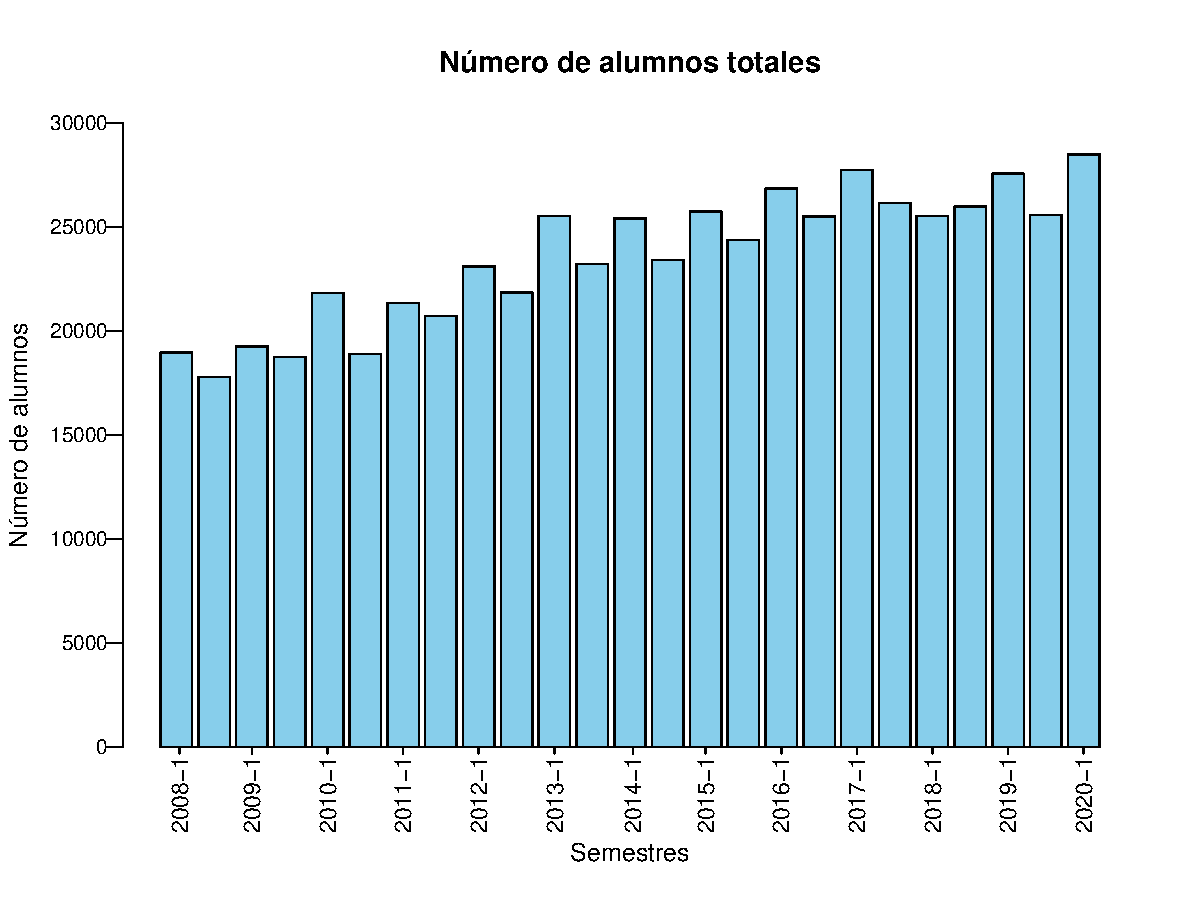
\includegraphics[width=\textwidth]{num_alum_total_x_sem_barplot} %scale = 0.8
\caption[\textit{Número total de alumnos por semestre}]{\textit{Número total de alumnos por semestre: En esta figura se muestra la gráfica de barras del número total de alumnos inscritos por cada semestre. Se observa que año con año el número aumenta. En general, el número de alumnos de los semestres impares es mayor que el de su respectivo semestre par.}}\label{TotalAlumBarras}
\end{figure}


Para probar que los datos tienen variación estacional utilizamos la función \verb@qs(X)@, de \textit{R}. Dicha función tiene como hipótesis nula $H_{0}:$ No hay estacionalidad en la serie de tiempo. En la \figurename{~\ref{QS_testSeasonality}} se muestran los resultados de la prueba QS. Podemos ver que \textit{p-value} $ = 1.473075 \times 10^{-06} \leqslant 0.01 = \alpha$ por lo tanto se rechaza $H_{0}$. Con ello concluimos que los datos tienen variación estacional.
%https://www.rdocumentation.org/packages/seasonal/versions/1.7.1/topics/summary.seas

\begin{figure}[H]
\centering
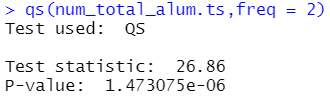
\includegraphics[scale = 1]{qs_test_seasonality} %width=\textwidth
\caption[\textit{Prueba QS para estacionalidad}]{\textit{Prueba QS para estacionalidad: En esta figura se muestran los resultados de la prueba QS. Esta prueba se utiliza para probar si los datos tienen estacionalidad.}}\label{QS_testSeasonality}
\end{figure}



\subsection{Prueba de homocedasticidad}

El término homocedasticidad se utiliza cuando algo tiene varianza constante. En nuestro caso, nos interesa probar que los datos con el número de alumnos totales tiene varianza constante. Ésto para comprobar que el modelo de estacionalidad adecuado para nuestros datos es el aditivo.

En la \figurename{~\ref{sd_alum_x_gpo_x_sem_ts}} se muestra la gráfica de la desviación estándar del número de alumnos por grupo y por semestre de todas las materias. Observamos que los valores se mantienen constantes a lo largo del tiempo, en un rango de entre 24 y 29 alumnos.


\begin{figure}[H]
\centering
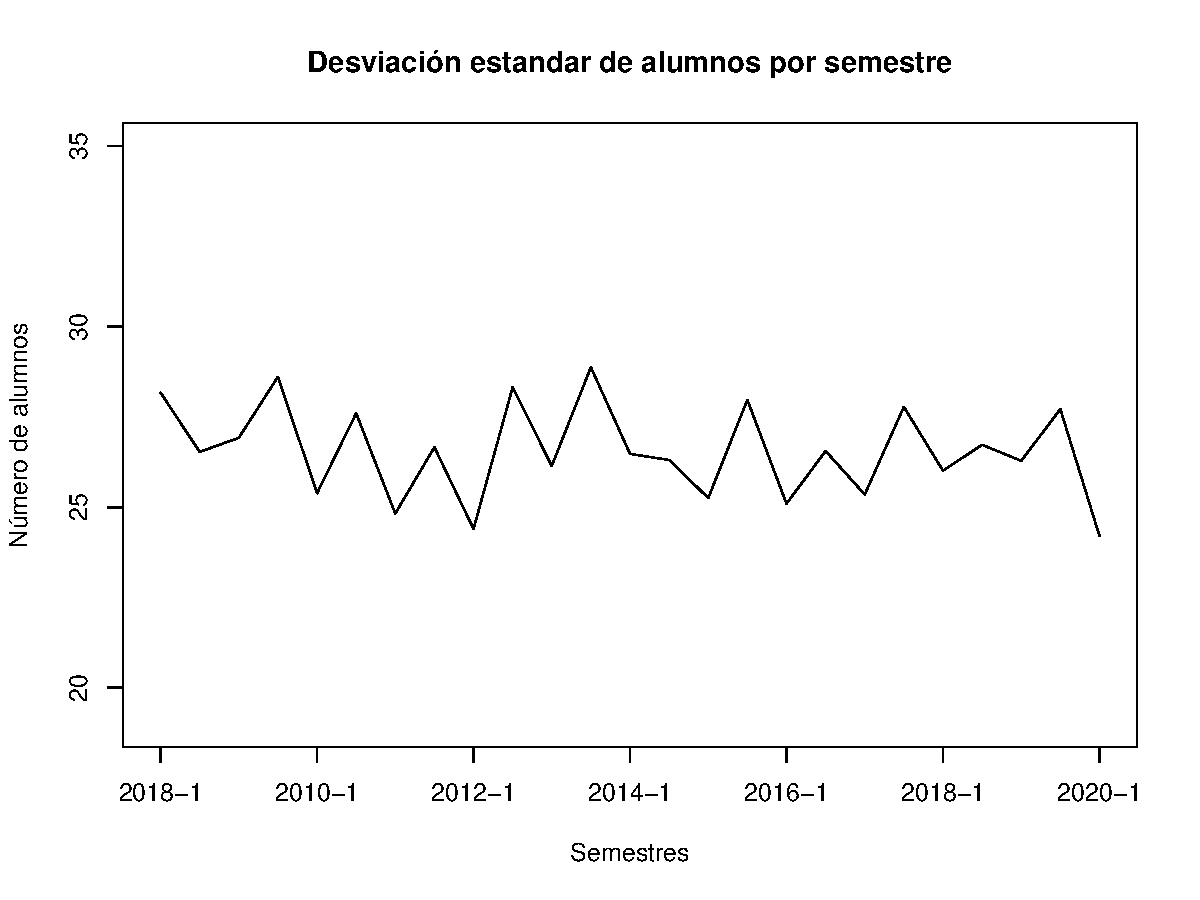
\includegraphics[scale = 0.7]{sd_alum_x_gpo_x_sem_ts.pdf} %width=\textwidth
\caption[\textit{Desviación estándar del número de alumnos por semestre}]{\textit{Desviación estándar del número de alumnos por semestre: Se muestra el comportamiento de los datos el cual es constante a lo largo del tiempo.}}\label{sd_alum_x_gpo_x_sem_ts}
\end{figure}



Utilizamos la prueba Breusch-Pagan que tiene como supuesto que los datos tienen una distribución normal. Para probar que los datos se distribuyen normal, utilizamos la prueba Jarque-Bera. El comando en \textit{R} es: \verb@jarque.bera.test(X)@. Dicha prueba tiene como hipótesis nula $H_{0}:$ Los datos provienen de una distribución normal.

En la \figurename{~\ref{JarqueBeraTest_normality}} vemos el resultado de la prueba Jarque-Bera. Notamos que \textit{p-value} $ = 0.4084 > 0.01 = \alpha$ por lo tanto no se rechaza $H_{0}$, entonces la distribución de los datos es normal.

\begin{figure}[H]
\centering
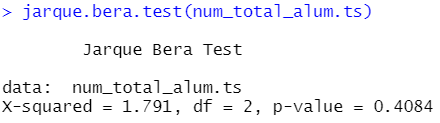
\includegraphics[scale = 1]{jarque_bera_test_normality} %width=\textwidth
\caption[\textit{Prueba Jarque-Bera para normalidad}]{\textit{Prueba Jarque-Bera para normalidad: En esta figura se muestran los resultados de la prueba Jarque-Bera. Esta prueba se utiliza para probar si los datos tienen una distribución normal.}}\label{JarqueBeraTest_normality}
\end{figure}


%Una vez que probamos el supuesto de normalidad en los datos, utilizamos la función \verb@bptest(lm(X~t))@.
Para probar la homocedasticidad de los datos, utilizamos la función \verb@bptest(lm(X~t))@. Esta función corresponde a la prueba Breusch-Pagan. El ajuste del modelo lineal con la función \verb@lm(X~t)@ es con respecto al tiempo. La prueba mencionada tiene como hipótesis nula $H_{0}:$ La varianza es constante.

En la \figurename{~\ref{bpTest_homocedasticidad}} Se muestra el resultado de la prueba. Vemos que \textit{p-value} $ = 0.8213 > 0.01 = \alpha$ por lo tanto no se rechaza $H_{0}$, entonces la varianza de los datos es constante.


\begin{figure}[H]
\centering
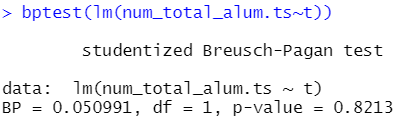
\includegraphics[scale = 1]{bp_test_homocedasticidad} %width=\textwidth
\caption[\textit{Prueba Breusch-Pagan para homocedasticidad}]{\textit{Prueba Breusch-Pagan para homocedasticidad: En esta figura se muestran los resultados de la prueba Breusch-Pagan. Esta prueba se utiliza para probar si los datos tienen varianza constante.}}\label{bpTest_homocedasticidad}
\end{figure}


Con las pruebas de tendencia y de estacionalidad confirmamos que se puede utilizar el método Holt-Winters. La prueba de homocedasticidad nos ayuda a verificar que el modelo de estacionalidad que debemos utilizar es el aditivo. Con estas observaciones concluímos que el método Holt-Winters aditivo es el método adecuado para poder hacer predicciones con nuestros datos.

\section{Análisis estadístico por grupo de datos} \label{AE_x_GpoDeDatos}

En la \figurename{~\ref{NumAlTotal_ParImpar_ts}} vemos la gráfica del número de alumnos separado por semestres pares e impares. Se observa un comportamiento similar al de la \figurename{~\ref{ParImparProbaI}}, de la Sección \ref{DatosAnalizar}. Vemos con mayor claridad lo que ocurre en la \figurename{~\ref{TotalAlumBarras}}, los datos efectivamente tienen una tendencia creciente. Notamos que el número de alumnos de los semestres impares es mayor al número total de alumnos de los semestres pares en todos los semestres, salvo en el semestre 2018-1 en donde el número de alumnos es menor a los de los semestres adyacentes.%, los cuales son el 2017-2 y el 2018-2.

\begin{figure}[H]
\centering
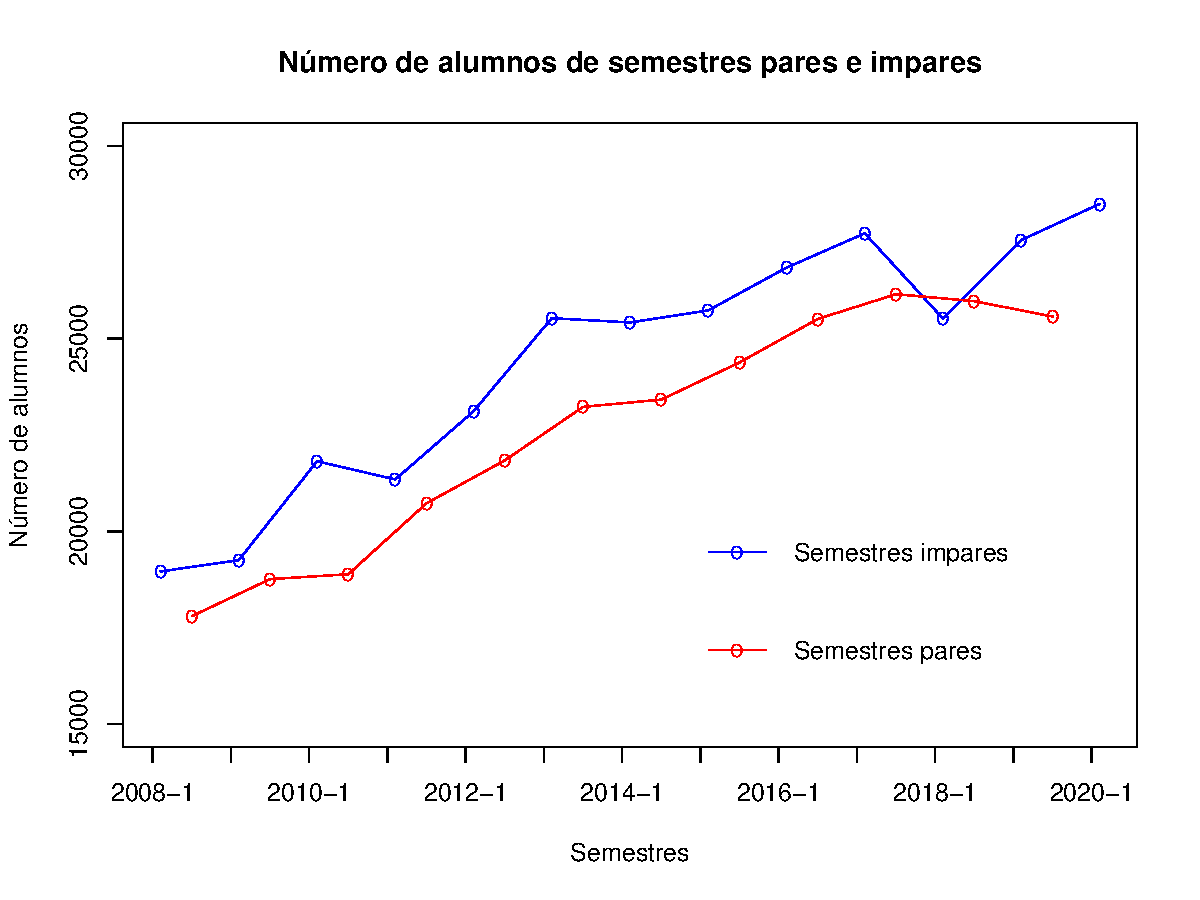
\includegraphics[scale = 0.7]{num_alum_sem_par_impar_ts.pdf} %width=\textwidth
\caption[\textit{Número de alumnos de semestres pares e impares}]{\textit{Número de alumnos de semestres pares e impares: Se observa una tendencia creciente y en general el número de alumnos de semestres impares (línea azul) es mayor al número de alumnos de semestres pares (línea roja).}}\label{NumAlTotal_ParImpar_ts}
\end{figure}


En la \figurename{~\ref{histNumAlTotal_ParImpar}} observamos los dos histogramas con el número total de alumnos de semestres pares e impares con sus respectivas densidades ajustadas. Notamos que hay una ligera diferencia entre el número de alumnos de los semestres pares con respecto al número de alumnos de los semestres impares. Existe una mayor cantidad de grupos en los semestres pares con un menor número de alumnos, que en los semestres impares. Hay una mayor cantidad de grupos en los semestres impares contra los semestres pares, que tienen entre 35 y 100 alumnos. Tanto para los semestres pares como para los impares, el comportamiento de las densidades ajustadas es muy parecido.

%\begin{figure}[H]
%\centering
%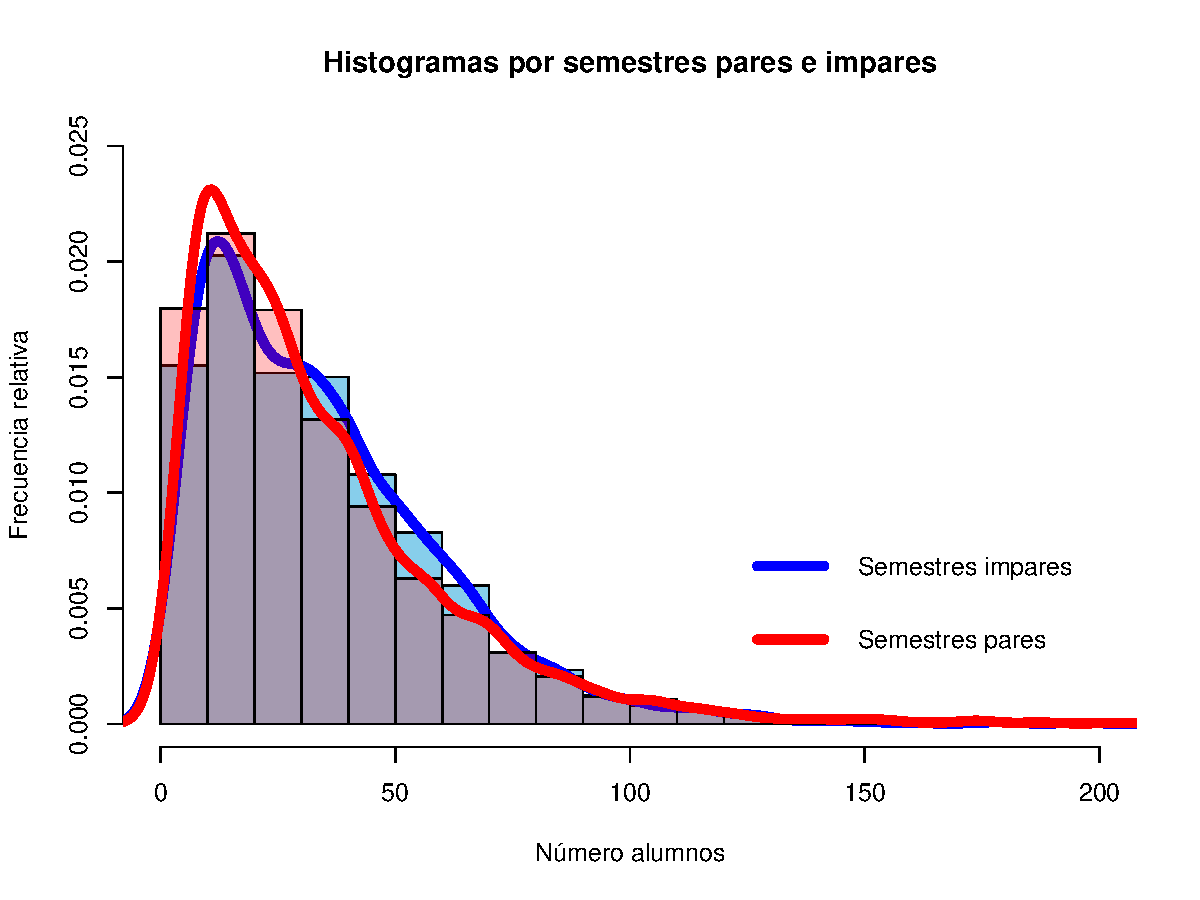
\includegraphics[scale = 0.65]{histograma_FR_num_alum_sem_par_impar.pdf} %width=\textwidth
%\caption[\textit{Histogramas del número de alumnos de semestres pares e impares}]{\textit{Histogramas del número de alumnos de semestres pares e impares: Las densidades ajustadas son muy parecidas, no importa si los datos son de semestres pares o impares.}}\label{histNumAlTotal_ParImpar}
%\end{figure}


En la \figurename{~\ref{NumAlTotal_MatuVesp_ts}} mostramos la gráfica del número de alumnos por turno: matutino y vespertino. Se puede observar que en todo momento el número de alumnos del turno matutino es mayor al número de alumnos del turno vespertino.

%\begin{figure}[H]
%\centering
%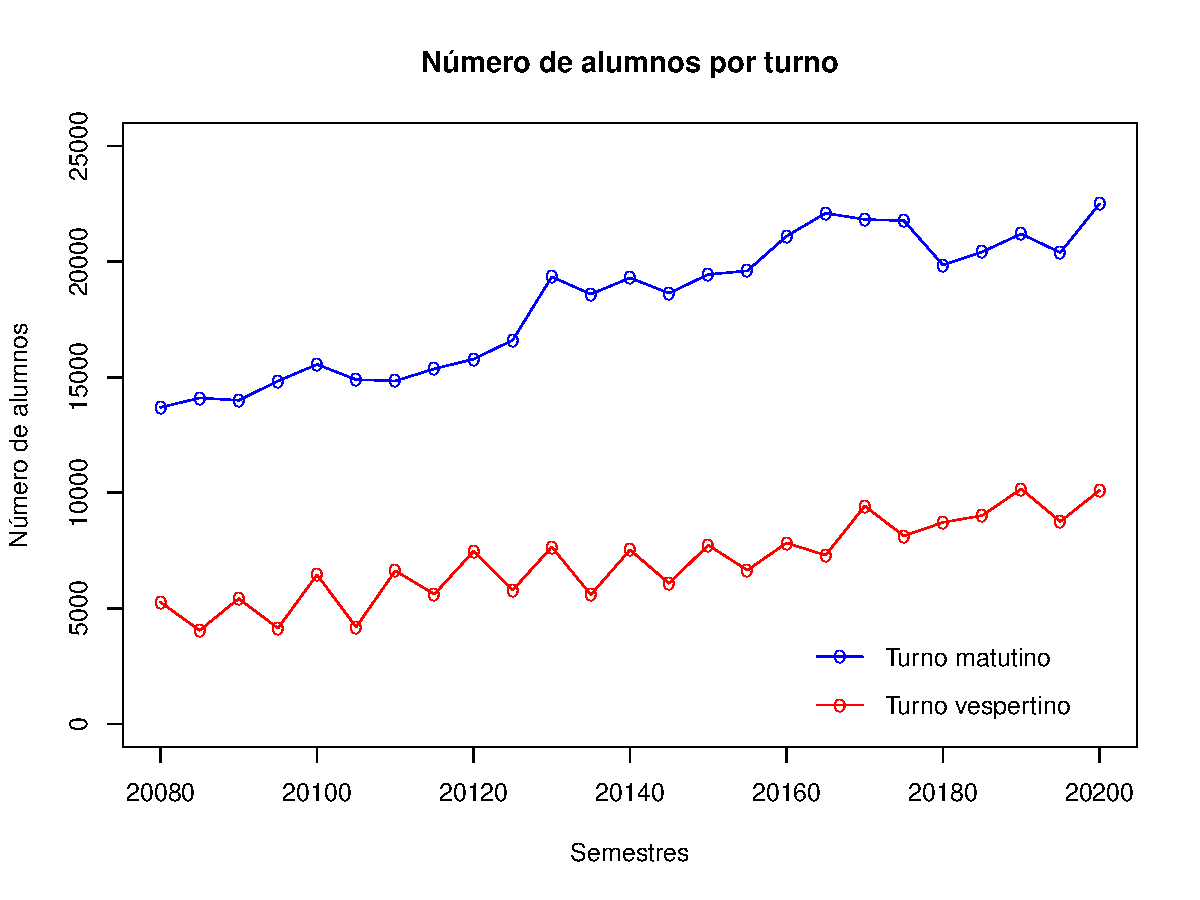
\includegraphics[scale = 0.7]{num_alum_matu_vesp_ts.pdf} %width=\textwidth
%\caption[\textit{Número de alumnos por turno de todos los semestres}]{\textit{Número de alumnos por turno de todos los semestres: Se observa que la línea azul (turno matutino) está en todo momento por encima de la línea roja (turno vespertino).}}\label{NumAlTotal_MatuVesp_ts}
%\end{figure}

Los datos que se graficaron en el histograma de la \figurename{~\ref{histNumAlTotal_MatuVesp}} son los alumnos totales por hora de cada semestre. En dicha figura se muestran los dos histogramas con los datos divididos en los turnos matutino y vespertino. Notamos que las densidades ajustadas de cada turno son completamente diferentes. Al ver la gráfica podemos concluir que hay más alumnos en el turno matutino que en el vespertino.

\begin{figure}[H]
\centering
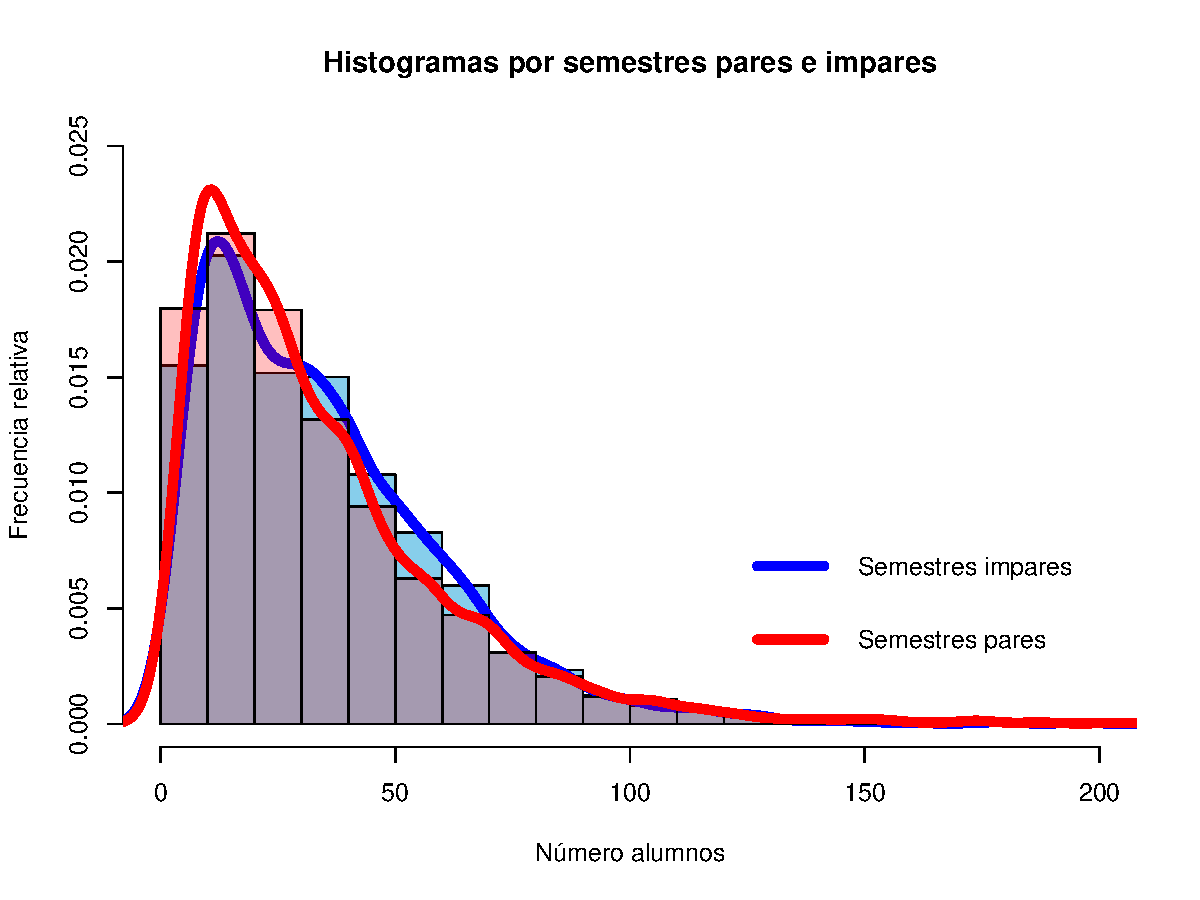
\includegraphics[scale = 0.65]{histograma_FR_num_alum_sem_par_impar.pdf} %width=\textwidth
\caption[\textit{Histogramas del número de alumnos de semestres pares e impares}]{\textit{Histogramas del número de alumnos de semestres pares e impares: Las densidades ajustadas son muy parecidas, no importa si los datos son de semestres pares o impares.}}\label{histNumAlTotal_ParImpar}
\end{figure}

\begin{figure}[H]
\centering
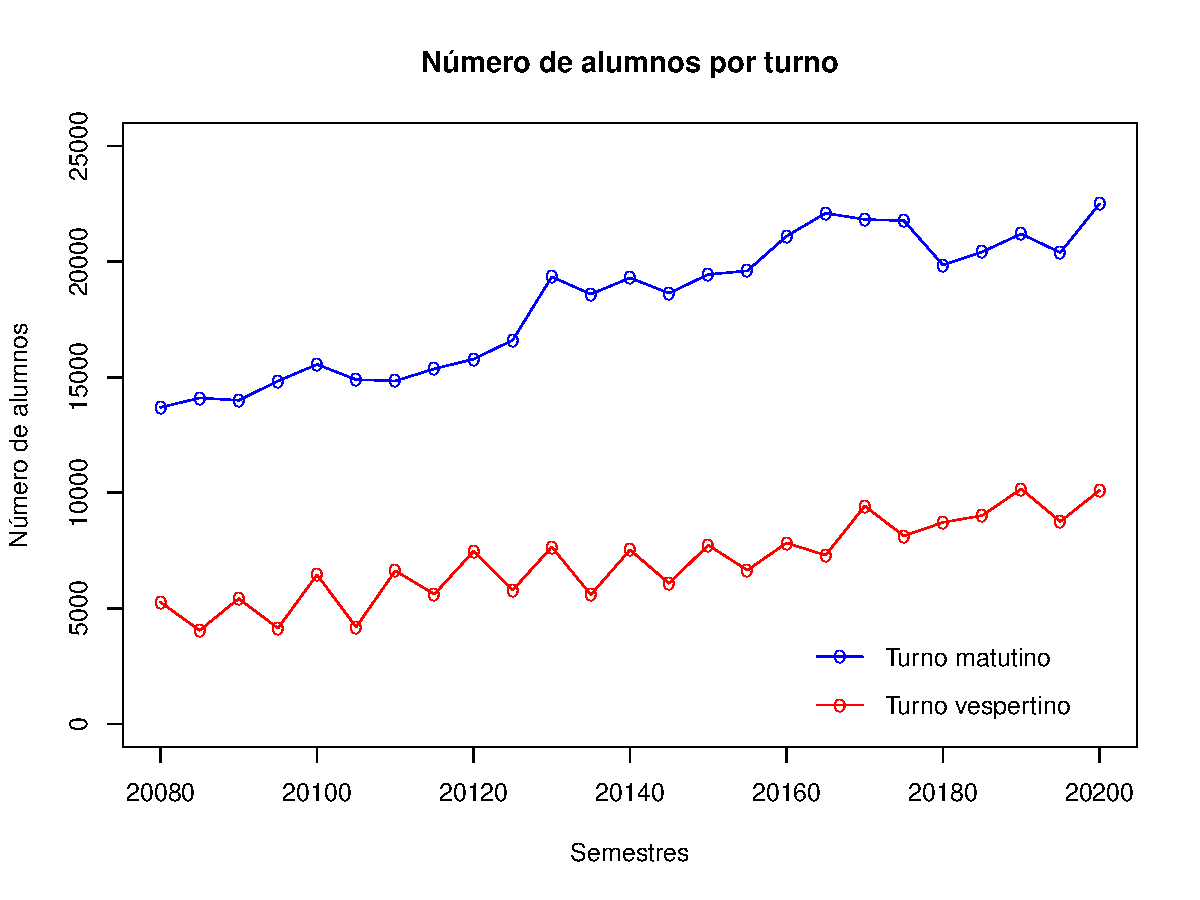
\includegraphics[scale = 0.7]{num_alum_matu_vesp_ts.pdf} %width=\textwidth
\caption[\textit{Número de alumnos por turno de todos los semestres}]{\textit{Número de alumnos por turno de todos los semestres: Se observa que la línea azul (turno matutino) está en todo momento por encima de la línea roja (turno vespertino).}}\label{NumAlTotal_MatuVesp_ts}
\end{figure}

\begin{figure}[H]
\centering
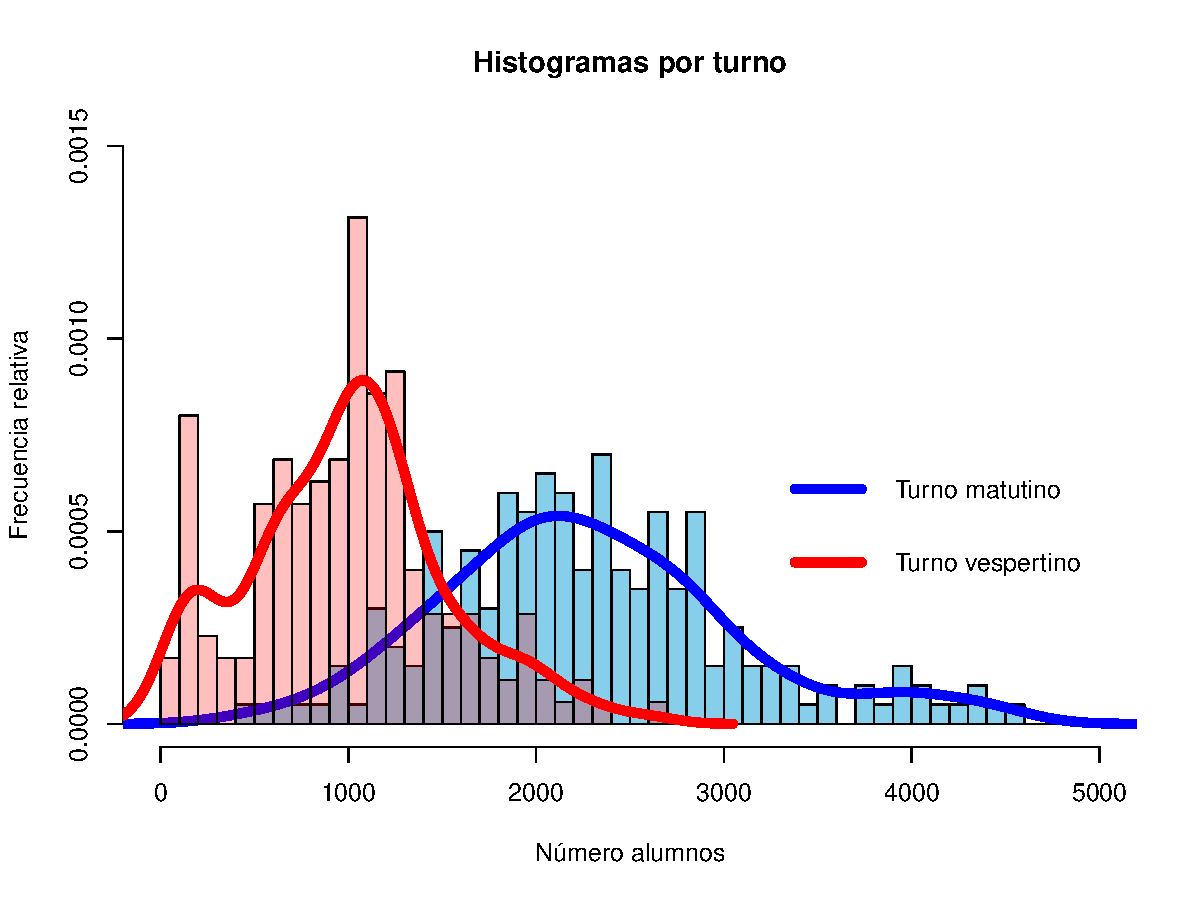
\includegraphics[scale = 0.65]{histograma_FR_num_alum_matu_vesp.pdf} %width=\textwidth
\caption[\textit{Histogramas del número de alumnos de los turnos matutino y vespertino}]{\textit{Histogramas del número de alumnos de los turnos matutino y vespertino: Al observar esta figura podemos concluir que hay más alumnos en el turno matutino que en el vespertino. Sus densidades ajustadas son diferentes.}}\label{histNumAlTotal_MatuVesp}
\end{figure}


\section{Análisis estadístico por carrera}

Es importante recordar que dentro de las carreras existe un tronco común. Es decir, comparten muchas de las materias impartidas en los primeros 4 semestres, por lo que muchos de los grupos de una carrera se encuentran en otra. Cabe mencionar que el número máximo de alumnos por grupo para la carrera de Ciencias de la Computación es 211 y para las otras carreras es 353.

En la \figurename{~\ref{histFAnumAl_x_carrera}} vemos cuatro histogramas con el número de alumnos por grupo, uno para cada carrera del Departamento de Matemáticas. La escala del eje $Y$ es igual para todos los histogramas. De esta manera podemos observar que en las carreras de Actuaría, Ciencias de la Computación y Matemáticas, se tiene la mayor concentración en los grupos de entre 10 y 20 alumnos. La carrera de Matemáticas Aplicadas tiene su mayor concesntración en los grupos que tienen entre 20 y 30 alumnos.

\begin{figure}[H]
\centering
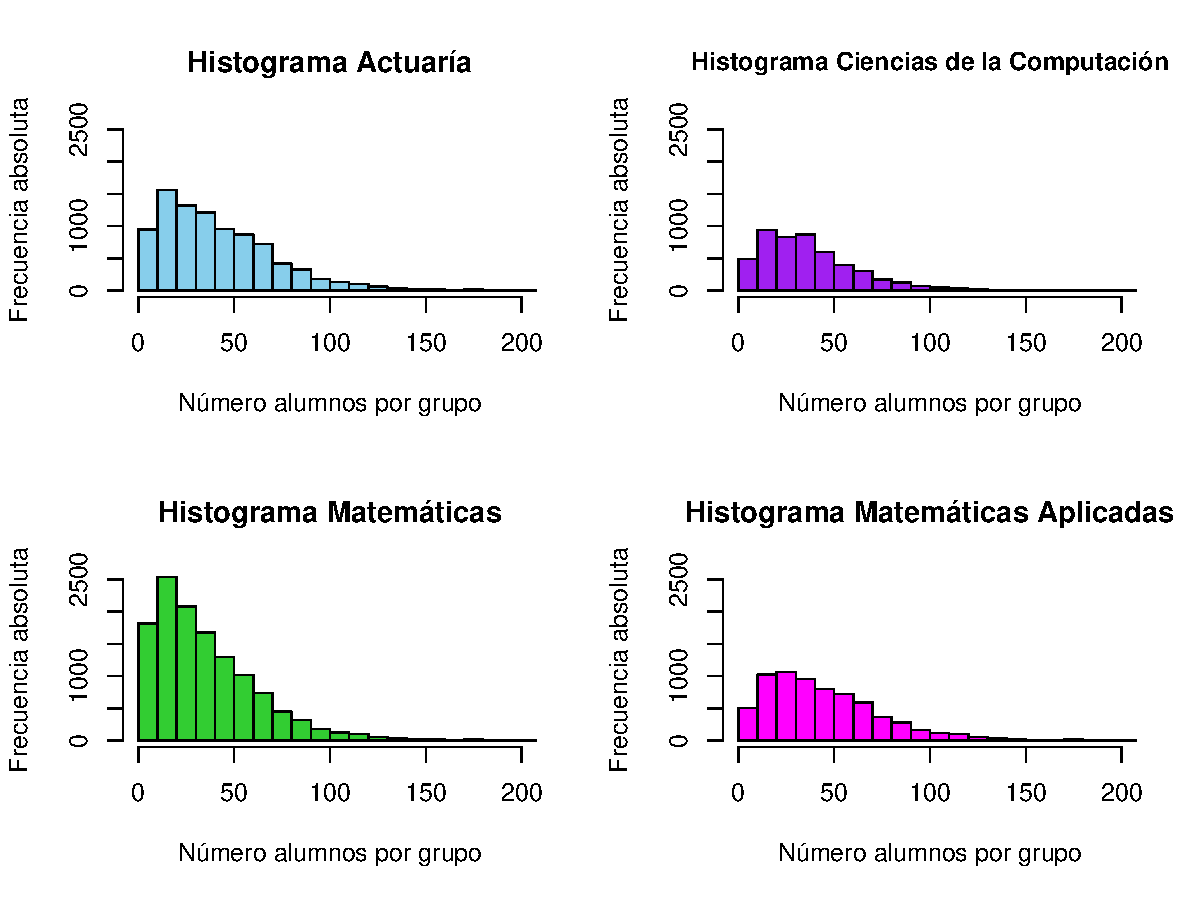
\includegraphics[width=\textwidth]{histogramas_FA_num_alum_x_carrera.pdf} %scale = 0.8
\caption[\textit{Histogramas del número de alumnos por carrera}]{\textit{Histogramas del número de alumnos por carrera: Se muestran los histogramas con el número de alumnos por grupo. Hay un histograma para cada carrera del Departamento de Matemáticas.}}\label{histFAnumAl_x_carrera}
\end{figure}


En la \figurename{~\ref{histFRnumAl_x_carrera}} vemos una gráfica con las densidades ajustadas a los datos del número de alumnos por grupos para cada carrera. Al ver la densidad ajustada a los datos de la carrera de Matemáticas vemos que tiene una mayor concentración de grupos que tienen aproximadamente entre 10 y 30 alumnos, a diferencia de las otras carreras. También podemos observar que en Actuaría y en Matemáticas Aplicadas hay una mayor concentración en los grupos que tienen aproximadamente entre 50 y 75 alumnos, que en Matemáticas o en Ciencias de la Computación. Si vemos la densidad ajustada a los datos de Ciencias de la Computación notamos que hay dos grandes concentraciones, una en los grupos de aproximadamente entre 20 y 30 alumnos y otra entre 40 y 50 alumnos. Con esta gráfica podemos ver con mayor claridad lo que observamos en la \figurename{~\ref{histFAnumAl_x_carrera}}, el comportamiento es similar para todas las carreras pero cada una tiene su propia distribución.

\begin{figure}[H]
\centering
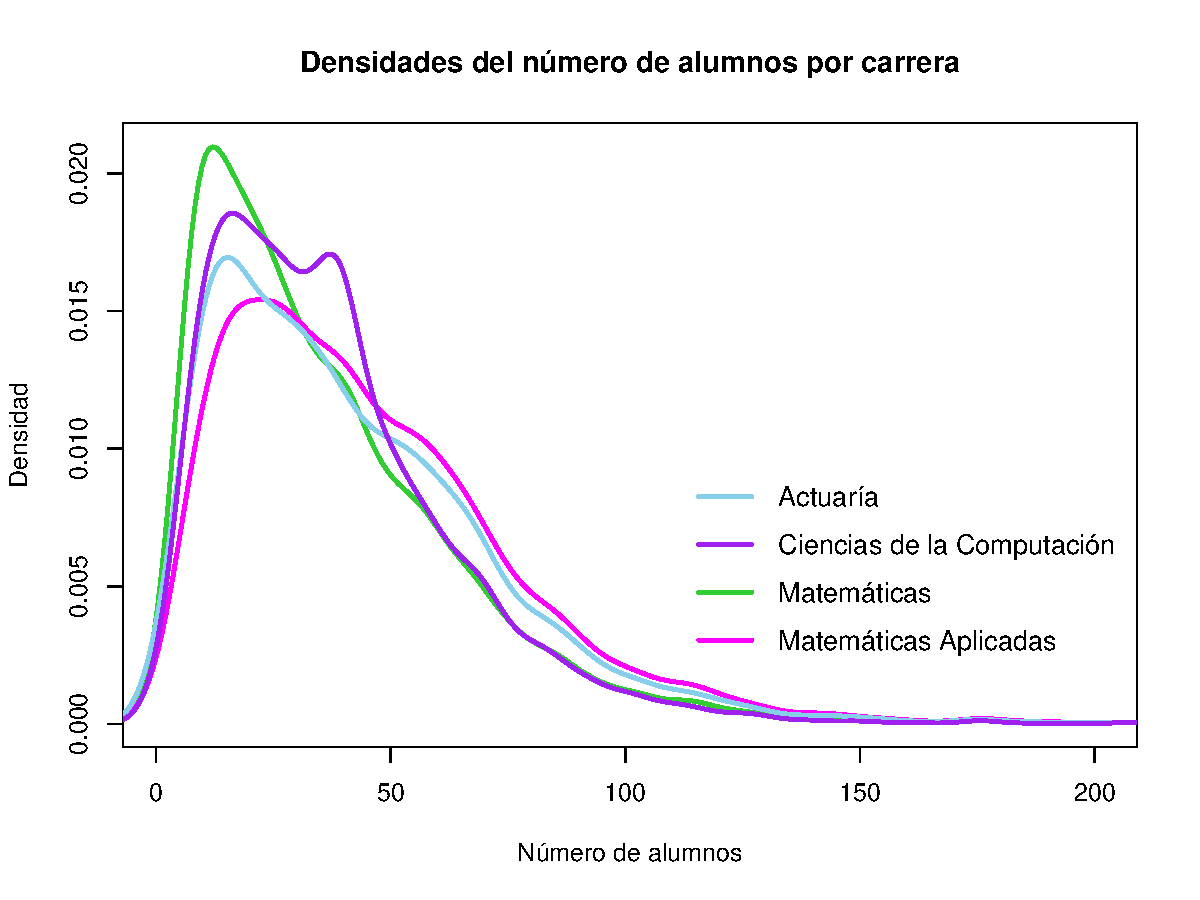
\includegraphics[scale = 0.7]{histogramas_FR_num_alum_x_carrera.pdf} %width=\textwidth
\caption[\textit{Densidades del número de alumnos por carrera}]{\textit{Densidades del número de alumnos por carrera: Se muestran las densidades ajustadas para cada carrera del Departamento de Matemáticas.}}\label{histFRnumAl_x_carrera}
\end{figure}


%\section{Distribución del número de alumnos por grupo / tamaño de grupo}
\section{Distribución del tamaño de los grupos} \label{DitribTamGpos}

En la \figurename{~\ref{histNumAl_x_gpo_x_sem}} se muestra el histograma del número de alumnos por grupo de todos los semestres, desde el 2008-1 hasta el 2020-1. Observamos el mismo comportamiento que en las Figuras \ref{histNumAlTotal_ParImpar}, \ref{histFAnumAl_x_carrera} y \ref{histFRnumAl_x_carrera}. La mayor frecuencia se encuentra en los grupos que tienen entre 10 y 20 alumnos.

%\begin{figure}[H]
%\centering
%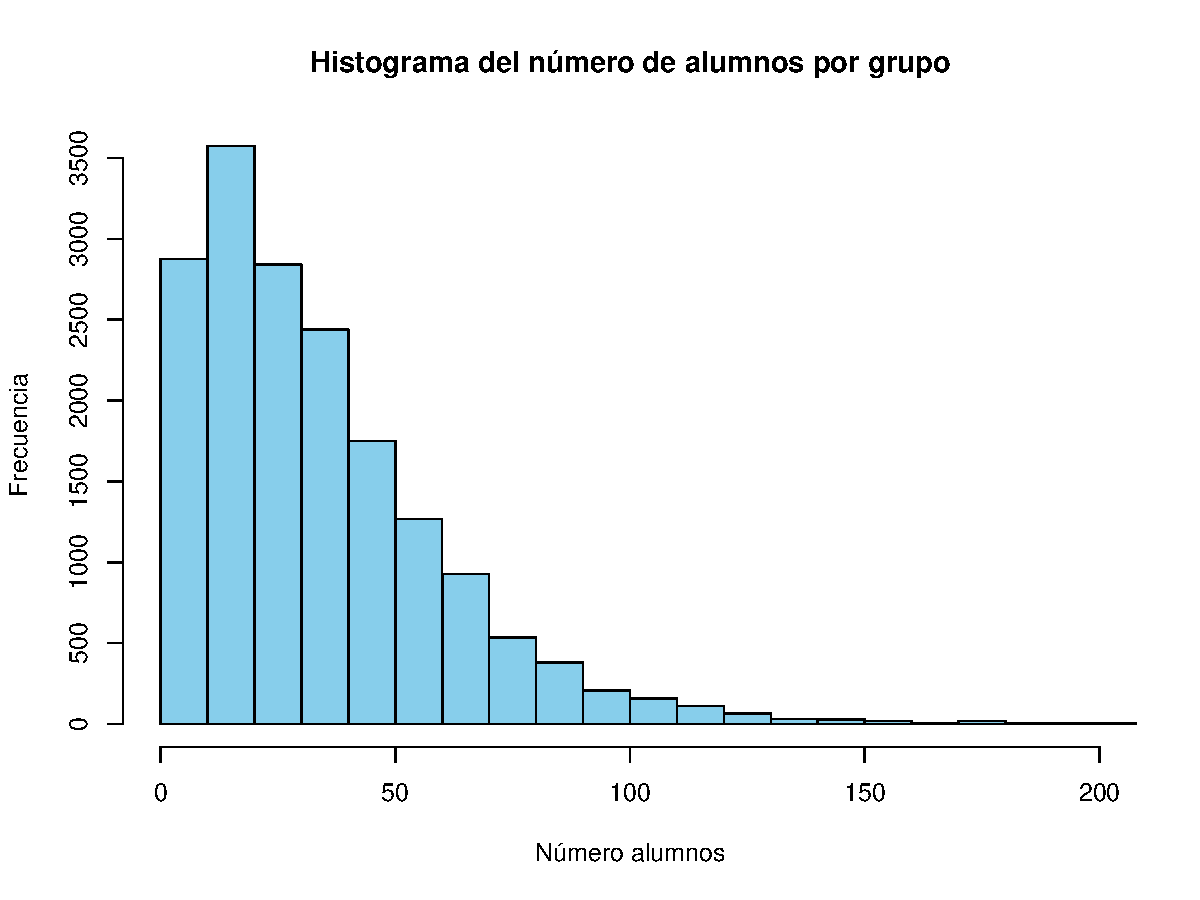
\includegraphics[scale = 0.7]{histograma_FA_num_alum_x_gpo_x_sem.pdf} %width=\textwidth
%\caption[\textit{Histograma del número de alumnos por grupo de todos los semestres}]{\textit{Histograma del número de alumnos por grupo de todos los semestres: La información es de los semestres del 2008-1 al 2020-1. Vemos una mayor concentración en los grupos que tienen entre 10 y 40 alumnos.}}\label{histNumAl_x_gpo_x_sem}
%\end{figure}


En la \figurename{~\ref{densidadesNumAl_x_gpo_x_sem}} vemos diferentes líneas con las densidades ajustadas a los valores del número de alumnos por grupo de cada semestre. Cada línea corresponde a un semestre. Se tomaron los datos de 25 semestres, del 2008-1 al 2020-1. Notamos que el comportamiento va cambiando conforme pasa el tiempo.

En dicha figura, las líneas de color verde corresponden a las densidades ajustadas a los datos de los semestres del 2008-1 al 2012-2. Las de color rosa corresponden a los semestres del 2013-1 al 2017-2. Las de color azul corresponden a los semestres 2018-1 al 2020-1.

Vemos que en los semestres más antiguos se tiene una concentración mayor en los grupos que tienen aproximadamente entre 10 y 30 alumnos. En los semestres más recientes la mayor concentración se tiene en los grupos con aproximadamente entre 25 y 50 alumnos. Esto lo podemos explicar con el hecho de que cada semestre incrementa el número de alumnos inscritos en la facultad, por lo tanto el tamaño de los grupos aumenta.

\begin{figure}[H]
\centering
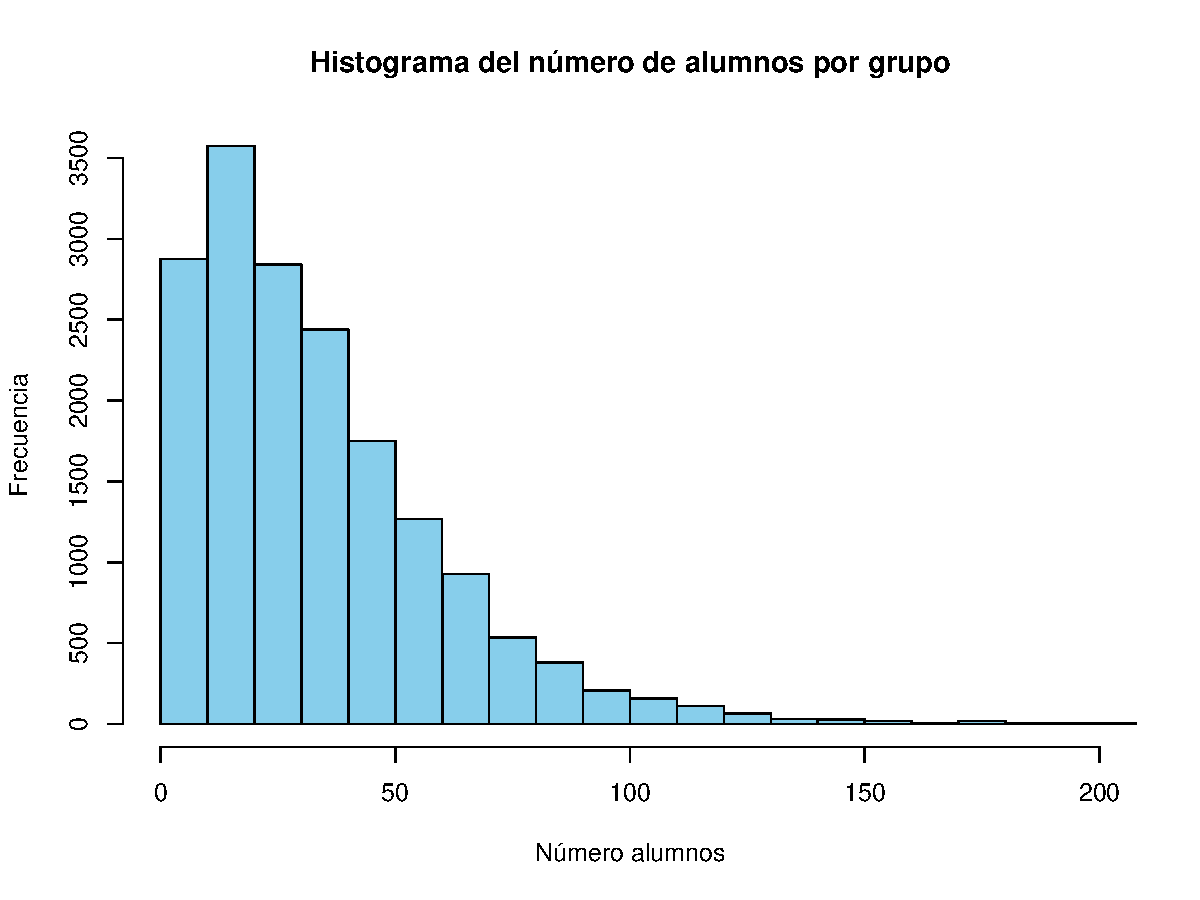
\includegraphics[scale = 0.65]{histograma_FA_num_alum_x_gpo_x_sem.pdf} %width=\textwidth
\caption[\textit{Histograma del número de alumnos por grupo de todos los semestres}]{\textit{Histograma del número de alumnos por grupo de todos los semestres: La información es de los semestres del 2008-1 al 2020-1. Vemos una mayor concentración en los grupos que tienen entre 10 y 40 alumnos.}}\label{histNumAl_x_gpo_x_sem}
\end{figure}

\begin{figure}[H]
\centering
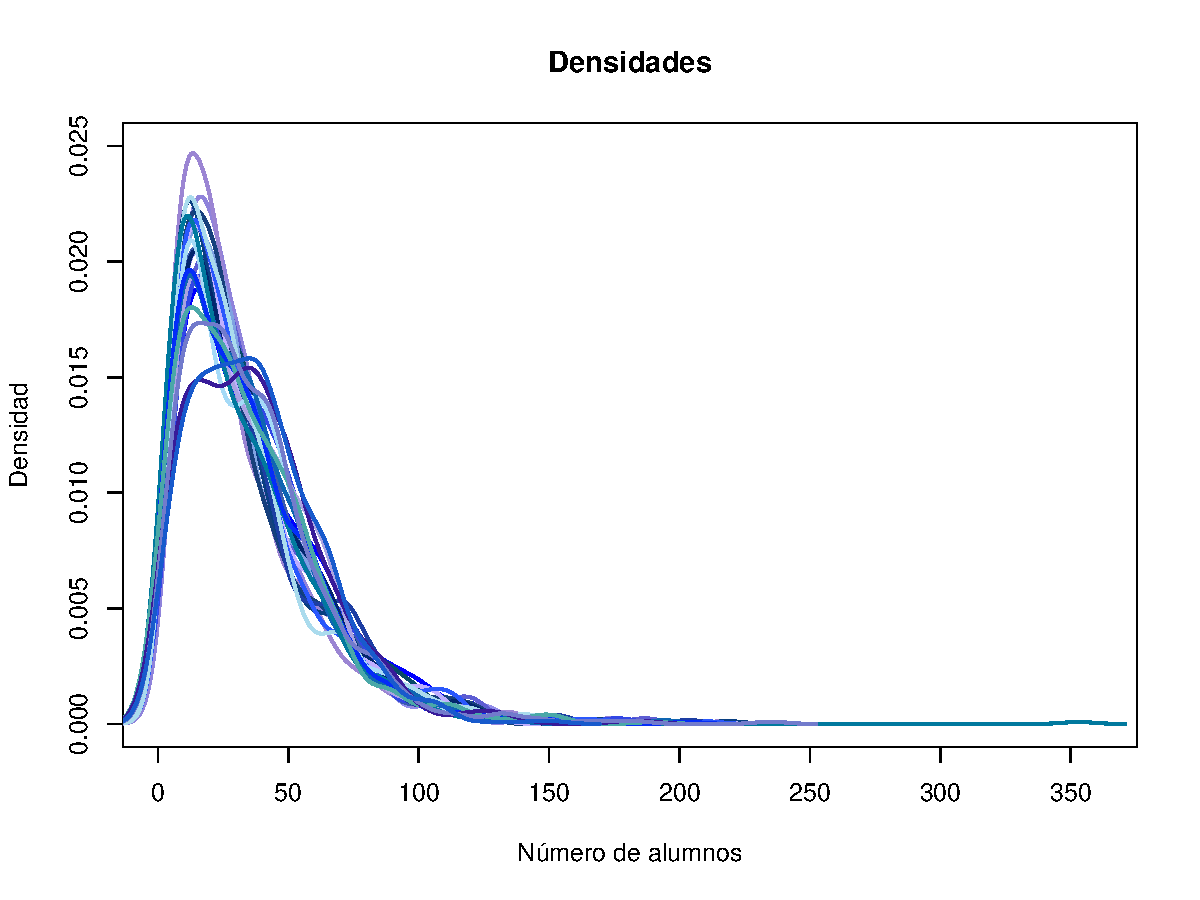
\includegraphics[scale = 0.7]{densidades_num_alum_x_gpo_x_sem.pdf} %width=\textwidth
\caption[\textit{Densidades del número de alumnos por grupo de cada semestre}]{\textit{Densidades del número de alumnos por grupo de cada semestre: Cada línea corresponde a la densidad ajustada de los datos de un semestre entre el 2008-1 y el 2020-1}}\label{densidadesNumAl_x_gpo_x_sem}
\end{figure}

También podemos observar que conforme pasa el tiempo la media y la varianza aumentan. Es decir, en semestres antiguos se tiene una menor media y varianza. Ésto comparado con los semestres más actuales, los cuales tienen una media y varianza mayor.

En los semestres del 2013-1 al 2017-2 se tuvieron grupos con más de 350 alumnos. En los semestres más recientes el número máximo de alumnos por grupo fue alrededor de 250. Esto lo podemos explicar por las medidas que se tomaron después del sismo del 19 de septiembre de 2017, con respecto al tamaño de los grupos. El número de alumnos inscritos no podía ser mayor al número de lugares disponibles por salón.

Viendo las Figuras \ref{histNumAl_x_gpo_x_sem} y \ref{densidadesNumAl_x_gpo_x_sem}, podríamos concluir que la distribución que mejor se ajusta al tamaño de los grupos es la distribución Poisson por la forma en la que están distribuidos los datos. Para probar esta hipótesis utilizamos la función \verb@ks.test(X,Y)@, de \textit{R}, para hacer la prueba de Kolmogorov-Smirnov.

La prueba de Kolmogorov-Smirnov, dice que se rechaza $H_{0}$ cuando $D_{n} > D_{n}^{1-\alpha}$. Donde $D_{n}^{1-\alpha}$ nos indica el valor en donde inicia la región de rechazo para un nivel de significancia de $\alpha$ y $n$ es el número de datos de la muestra. Tomamos como hipótesis nula $H_{0}: X$ y $Y$ tienen la misma distribución.

Definimos a $X$ como el vector con el número de alumnos por cada grupo del semestre 2008-1 al 2020-1. Definimos a $Y$ como un vector de números aleatorios de una distribución $Poisson(\lambda)$. Por el resultado \ref{EMVlambda}, del apéndice \ref{Apend_ResultadosUtiles}, sabemos que el estimador máximo verosímil de $\lambda$ para la distribución $Poisson(\lambda)$ es la media de los datos. Con este estimador $(\hat{\lambda} = 34.18),$ obtuvimos los números aleatorios de $Y$. Tenemos que $Y \sim Poisson(34.18)$.%\hat{\lambda} = 34.18746

Por [\ref{Miller}] sabemos que:
  
  \begin{equation}\label{Dn_KS}
D_{n}^{1-\alpha} = \sqrt{\dfrac{ln \left(\dfrac{1}{\alpha}\right)}{2n}} - 1.6693 n^{-1} - 0.20562 n^{-\frac{3}{2}}
\end{equation}

En nuestro caso los valores de las variables son: $n = 17,246$ y $\alpha = 0.01$. Sustituyendo en la ecuación \ref{Dn_KS} tenemos que $D_{17246}^{0.99} = 0.01$. Con la función \verb@ks.test(X,Y)@, de \textit{R}, obtenemos el valor de $D_{17246} = 0.39$.

Como $D_{17246} = 0.39 > 0.01 = D_{17246}^{0.99}$, entonces se rechaza $H_{0}$, por lo tanto los datos no siguen una distribución Poisson con $\lambda = 34.18$.


Hicimos otra prueba suponiendo que los datos tienen una distribución $Normal(\mu,\sigma)$. Para simular los datos de $Y$ utilizamos los estimadores máximo verosímiles de $\mu$ y $\sigma$. Estos estimadores los obtuvimos con la función \verb@fitdistr(X, densfun="normal")@, en \textit{R}. Los valores de los estimadores son $\hat{\mu} = 34.18$ y $\hat{\sigma} = 26.57$. El resultado de la función de la prueba de Kolmogorov-Smirnov es $D_{17246} = 0.10$.

Como $D_{17246} = 0.10 > 0.01 = D_{17246}^{0.99}$, entonces se rechaza $H_{0}$, por lo tanto los datos no siguen una distribución $Normal(34.18,26.57)$.

Hicimos más pruebas con otras distribuciones y en todos los casos rechazamos la hipótesis nula. En la \figurename{~\ref{histFR_pruebaKS}} vemos únicamente los casos que expusimos en esta sección. El histograma representa las frecuencias relativas de los datos del número de alumnos por grupo para cada semestre. La línea azul es la densidad ajustada generada por \textit{R}, la línea morada es la densidad de $n$ números aleatorios con distribución  $Poisson(34.18)$ y la línea roja es la densidad de $n$ números aleatorios con distribución  $Normal(34.18,26.57)$.

%Hicimos más pruebas con otras distribuciones y en todos los casos rechazamos la hipótesis nula. Con estos resultados concluímos que el ajuste que se pudiera hacer a los datos tendría que ser en dos partes. Un ejemplo de una posible partición de los datos es que se puede ajustar una distribución para los datos que están entre 0 y 100, y otra distribución para los datos mayores a 100. Esto debido a que a pesar de ser pocos los datos mayores a 100, si impactan en la distribución total. El análisis con esta propuesta no lo realizamos para este trabajo.

\begin{figure}[H]
\centering
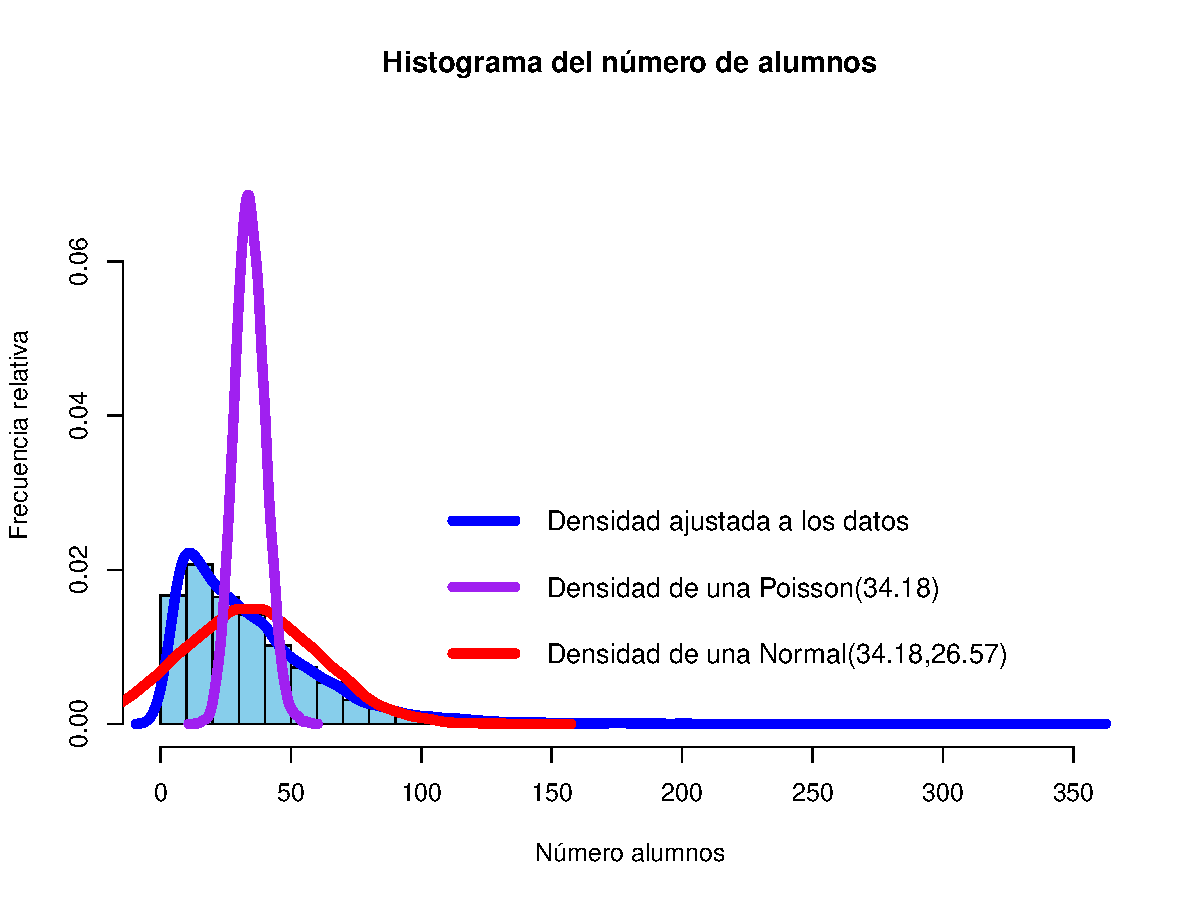
\includegraphics[scale = 0.8]{histograma_FR_prueba_KS.pdf} %width=\textwidth
\caption[\textit{Histograma con densidades ajustadas}]{\textit{Histograma con densidades ajustadas: Se muestran 3 densidades ajustadas. La línea azul es la ajustada con el método kernel gaussiano por la función $\mathrm{density()}$. La morada corresponde a una Poisson(34.18). La roja corresponde a una Normal(34.18,26.57). Ninguna de las distribuciones propuestas se ajustan de manera adecuada a los datos.}}\label{histFR_pruebaKS}
\end{figure}

%Hicimos más pruebas con otras distribuciones y en todos los casos rechazamos la hipótesis nula. Con estos resultados concluímos que el ajuste que se pudiera hacer a los datos tendría que ser en dos partes. Un ejemplo de una posible partición de los datos es que se puede ajustar una distribución para los datos que están entre 0 y 100, y otra distribución para los datos mayores a 100. Esto debido a que a pesar de ser pocos los datos mayores a 100, si impactan en la distribución total. El análisis con esta propuesta no lo realizamos para este trabajo.


\section{Comportamientos por hora}

En esta sección veremos algunas gráficas cuyo eje $x$ corresponde a las horas en las que se imparten las clases. Se empieza por la clase de 7-8hrs y se termina con la clase de 21-22hrs. Primero mostraremos el comportamiento del promedio de grupos por hora y después el comportamiento del promedio del número de alumnos por hora.

En la \figurename{~\ref{num_prom_gpos_x_hora_barplot}} vemos la gráfica de barras con el número promedio de grupos por hora. Tomamos la información de 25 semestres. Observamos una disminución considerable del número de grupos a las 15hrs. Podemos concluir que es debido a que a esa hora, usualmente la gente sale a comer. A las 21hrs se tiene el menor número de grupos, esto se puede explicar por el hecho de que es la última clase impartida en la Facultad.

Hay un descenso leve a las 9hrs donde se pudiera suponer que la gente sale a desayunar. Desde las 7hrs se pueden encontrar clases como \textit{Cálculo Diferencial e Integral}. Pero en general, las clases impartidas a las 7hrs y a las 8hrs suelen ser materias exclusivas para los actuarios como \textit{Teoría del Seguro, Matemáticas Actuariales del Seguro de Personas I y II} o \textit{Matemáticas Actuariales para Seguro de Daños, Fianzas y Reaseguro}. Podemos decir que a partir de las 9 de la mañana se imparten materias de todas las carreras.

%Hay un descenso leve a las 9hrs donde se pudiera suponer que la gente sale a desayunar. En mi caso particular, al estudiar la carrera de Actuaría, tenía clases desde las 7a.m. por lo que las 9a.m. era una buena hora para hacer una pequeña pausa en el horario y tener un descanso para desayunar. Esta hora coincide con el cambio en el que se dejan de impartir las materias exclusivas para los actuarios como Teoría del Seguro, MASP o MASD. Es decir, a partir de las 9 de la mañana se imparten materias de todas las carreras.

A las 10 de la mañana se tiene el número máximo de grupos. Con esta información se podría medir la capacidad que debería de tener la Facultad en cuanto al número de salones necesarios para cubrir la demanda de grupos. Si se está preparado para cubrir la demanda del pico más alto de todas las horas, entonces los demás casos están cubiertos por tener un menor número de grupos.


\begin{figure}[H]
\centering
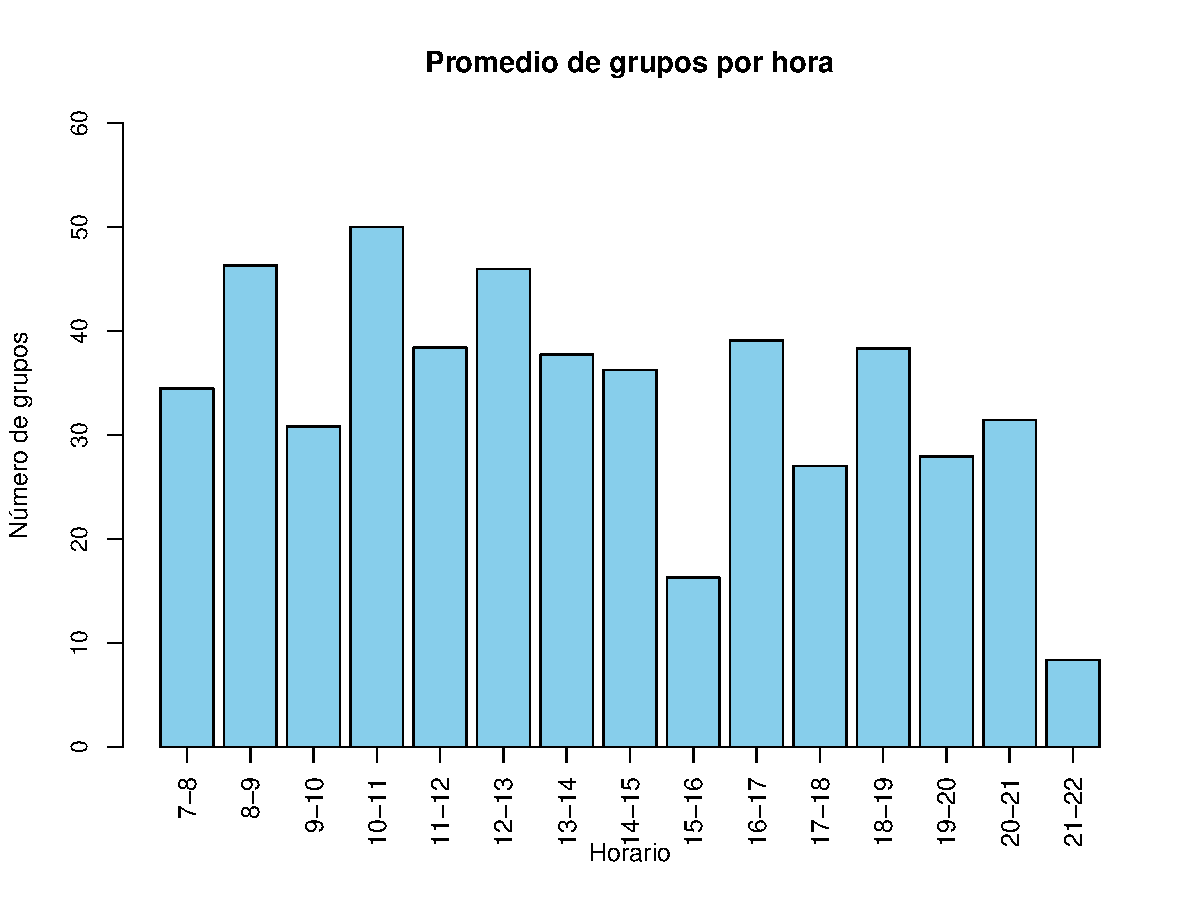
\includegraphics[scale = 0.8]{num_prom_gpos_x_hora_barplot.pdf} %width=\textwidth
\caption[\textit{Número promedio de grupos por hora}]{\textit{Número promedio de grupos por hora: Se observa una disminución considerable a las 15hrs y a las 21hrs. El valor más alto se encuentra a las 10hrs.}}\label{num_prom_gpos_x_hora_barplot}
\end{figure}

En la \figurename{~\ref{prom_alum_x_hora_barplot}} se muestra la gráfica de barras con el promedio del número de alumnos por hora. Notamos que el comportamiento de ésta gráfica es muy similar al de la gráfica mostrada en la \figurename{~\ref{num_prom_gpos_x_hora_barplot}}. El pico más alto de los datos también se tiene a las 10 de la mañana y el menor número de alumnos se encuentra a las 21hrs. También hay una disminución considerable a las 15hrs.

\begin{figure}[H]
\centering
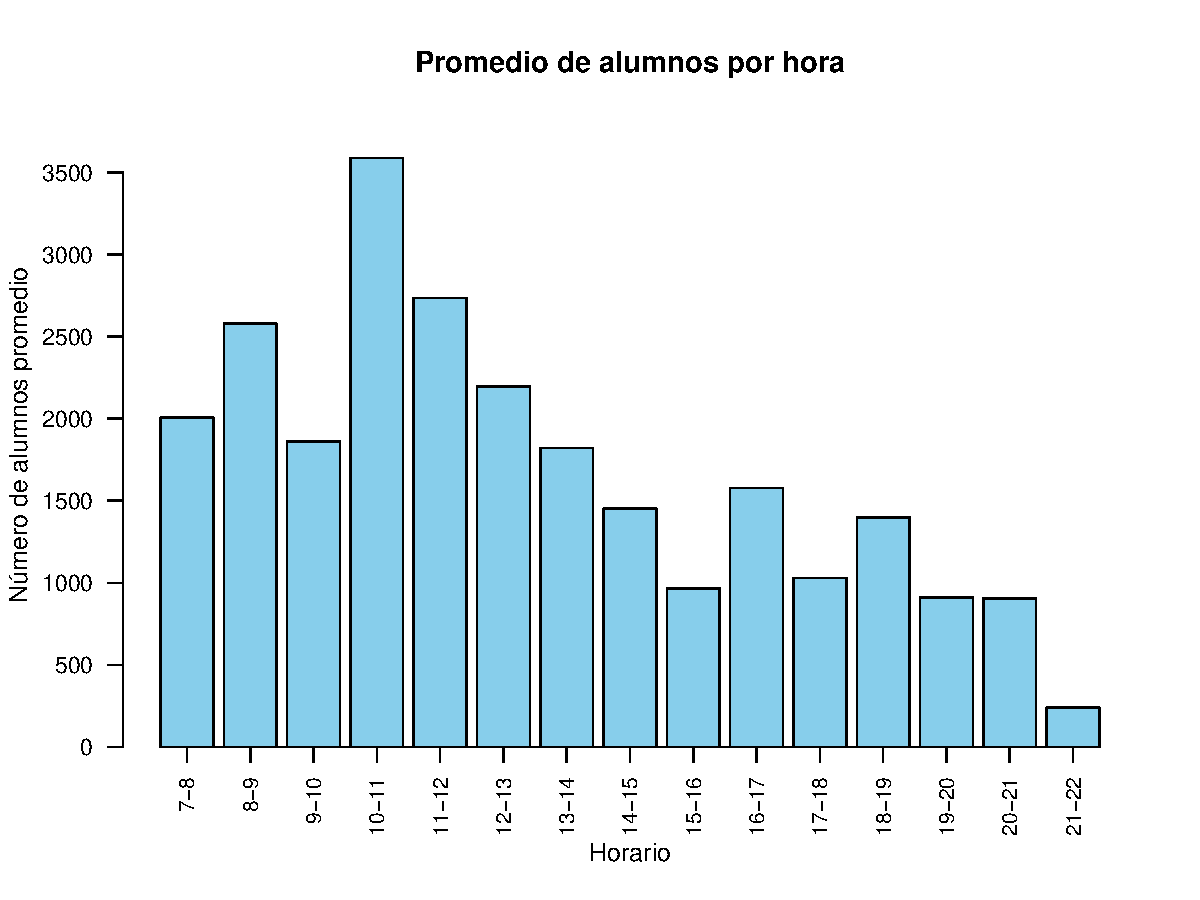
\includegraphics[scale = 0.8]{prom_alum_x_hora_barplot.pdf} %width=\textwidth
\caption[\textit{Número promedio de alumnos por hora}]{\textit{Número promedio de alumnos por hora: Notamos una disminución de los valores a las 9hrs, a las 15hrs y a las 21hrs. El valor más alto lo encontramos a las 10hrs.}}\label{prom_alum_x_hora_barplot}
\end{figure}

Viendo las Figuras \ref{num_prom_gpos_x_hora_barplot} y \ref{prom_alum_x_hora_barplot} podemos concluir que existe una correlación entre el número promedio de grupos por hora y el número promedio de alumnos por hora. Por ejemplo, si no hay alumnos que tomen clases a las 15hrs entonces no tiene caso que se abran grupos a esa hora. Análogamente para las 21hrs. Por el contrario entre más alumnos haya por hora, se deben abrir más grupos a esas horas, como es el caso de las 10hrs.